\documentclass[10pt,a4paper]{article}
\usepackage[utf8]{inputenc}
\usepackage[russian]{babel}
\usepackage[OT1]{fontenc}
\usepackage{amsmath}
\usepackage{amsfonts}
\usepackage{amssymb}
\usepackage{graphicx}
\DeclareGraphicsExtensions{.pdf,.png,.jpg}
\usepackage[left=2cm,right=2cm,top=2cm,bottom=2cm]{geometry}

\begin{document}
$\int_0^\infty \frac{e^{-z}}{(1 - x z)}\;\mathrm{d}z = \frac{e^{-1/x} \left(\text{Chi}\left(\frac{1}{x}\right)+\text{Shi}\left(\frac{1}{x}\right)-\log \left(\frac{1}{x}\right)-\log (-x)\right)}{x},\Im(x)\neq 0\lor \Re(x)\leq 0$\\

Как видно из графиков максимальное значение интеграла $\approx$ 1.92 и достигается при $x=-0,054$
При $x>-0,054$ значение интеграла 0
При $x<-0.054$ значение будет "осциллировать" с убывающей амплитудой, а "среднее" будет просто убывать, стремясь к 0 
\begin{figure}[h]
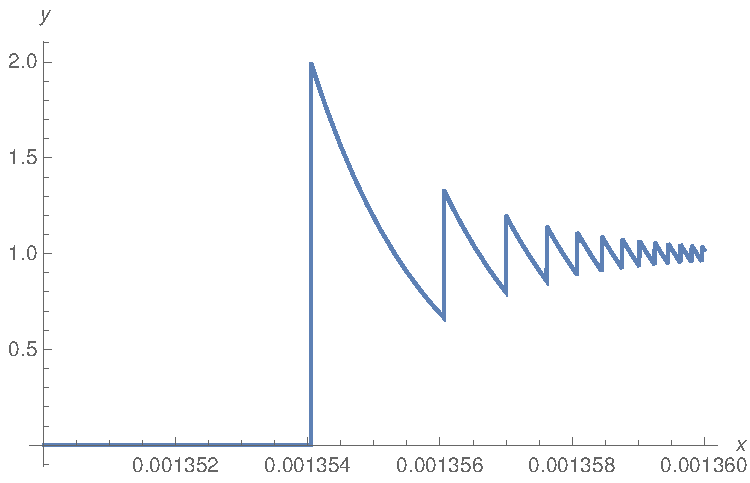
\includegraphics{gr1}
\end{figure}

\begin{figure}[h]
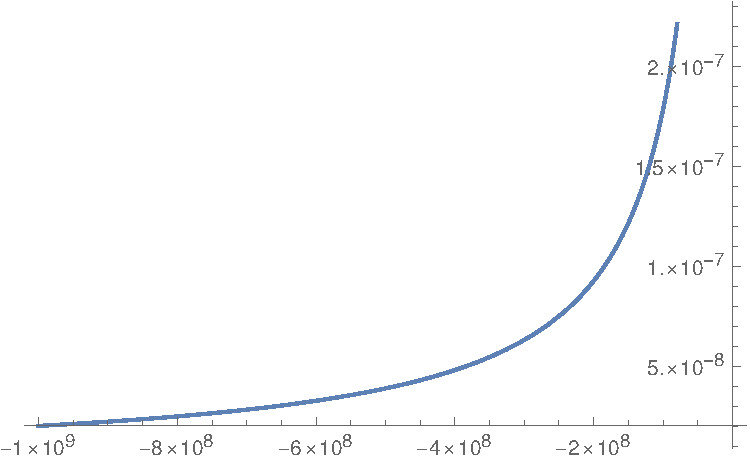
\includegraphics{gr2}
\end{figure}

\begin{figure}[!h]
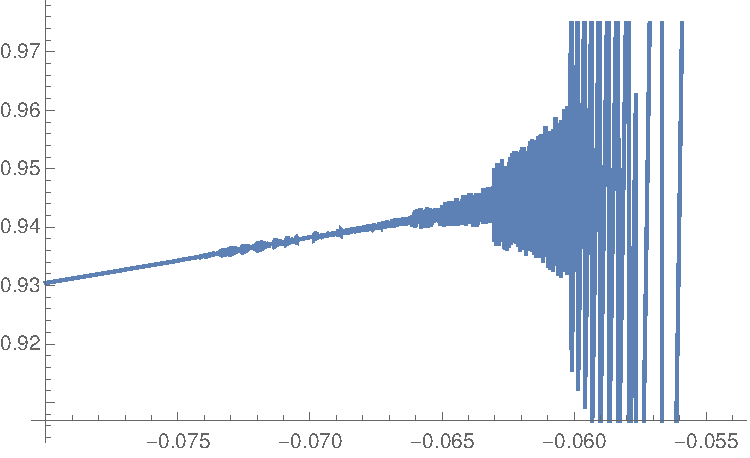
\includegraphics{gr3}
\end{figure}

$\int_{-\infty }^{\infty } e^{-x z^4-z^2} \, dz = \frac{e^{\frac{1}{8 x}} K_{\frac{1}{4}}\left(\frac{1}{8 x}\right)}{2 \sqrt{x}},\Re(x)>0$\\

Как видно из графиков максимальное значение интеграла $\approx$ 3.68 при $x\approx 0.0001684$\\
При $x<$ значения максимума значение интеграла равно 0\\
При $x>$ значения максимума значение интеграла начинает "осциллировать", а "среднее" будет убывать, стремясь к 0

\begin{figure}[h]
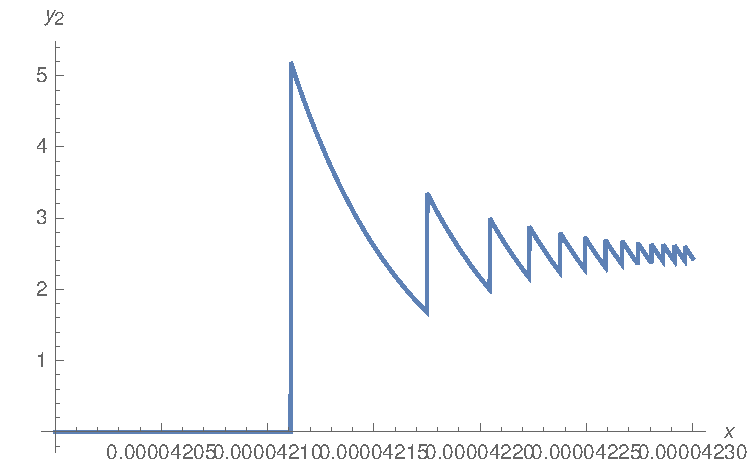
\includegraphics{gr4}
\end{figure}

\begin{figure}[h]
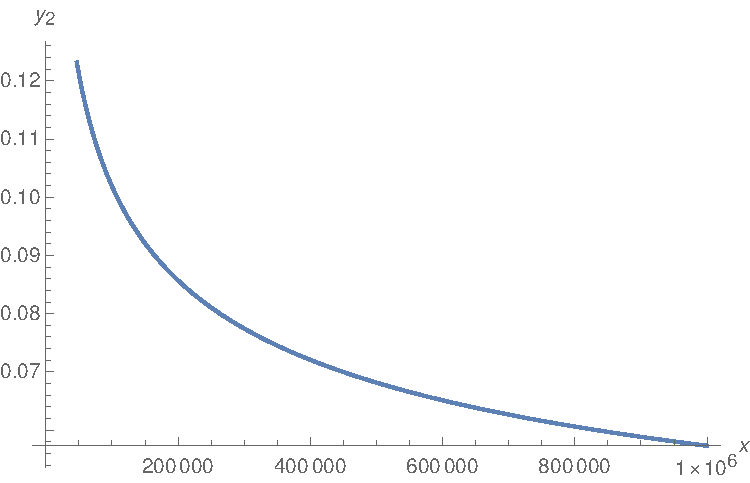
\includegraphics{gr5}
\end{figure}
\end{document}